
\begin{frame}{Diffuse Reflection - Introduction}
  \begin{columns}
    \begin{column}{0.7\textwidth}
      \begin{conceptbox}{Lambertian Surfaces}
        \small
        \textbf{Examples:}

        Paper, wood, fabric

        \vspace{0.3cm}
        \textbf{Characteristics:}
        \begin{itemize}
          \item Surface appears equally bright from all viewing angles
          \item Light scattered uniformly in all directions
          \item Brightness depends only on angle of incident light
        \end{itemize}
      \end{conceptbox}
    \end{column}
    \begin{column}{0.3\textwidth}
      \begin{tikzpicture}[scale=0.8]
        \draw[ObjectColor, very thick] (-2,0) -- (2,0);
        \fill[ObjectColor] (0,0) circle (3pt);
        \draw[->, PrimaryColor, thick] (0,0) -- (0,1.5) node[above] {\footnotesize $\mathbf{N}$};

        \draw[->, lightray, thick] (-1.5,1.5) -- (0,0);
        \node[above] at (-0.75,0.75) {\footnotesize $\mathbf{L}$};

        \foreach \angle in {30,60,90,120,150} {
          \draw[reflectray, opacity=0.6] (0,0) -- (\angle:1);
        }

        \node[below] at (0,-0.5) {\footnotesize Equal brightness};
        \node[below] at (0,-0.8) {\footnotesize all directions};
      \end{tikzpicture}
      \pause
      \vspace{0.3cm}
      \begin{center}
        \begin{figure}
          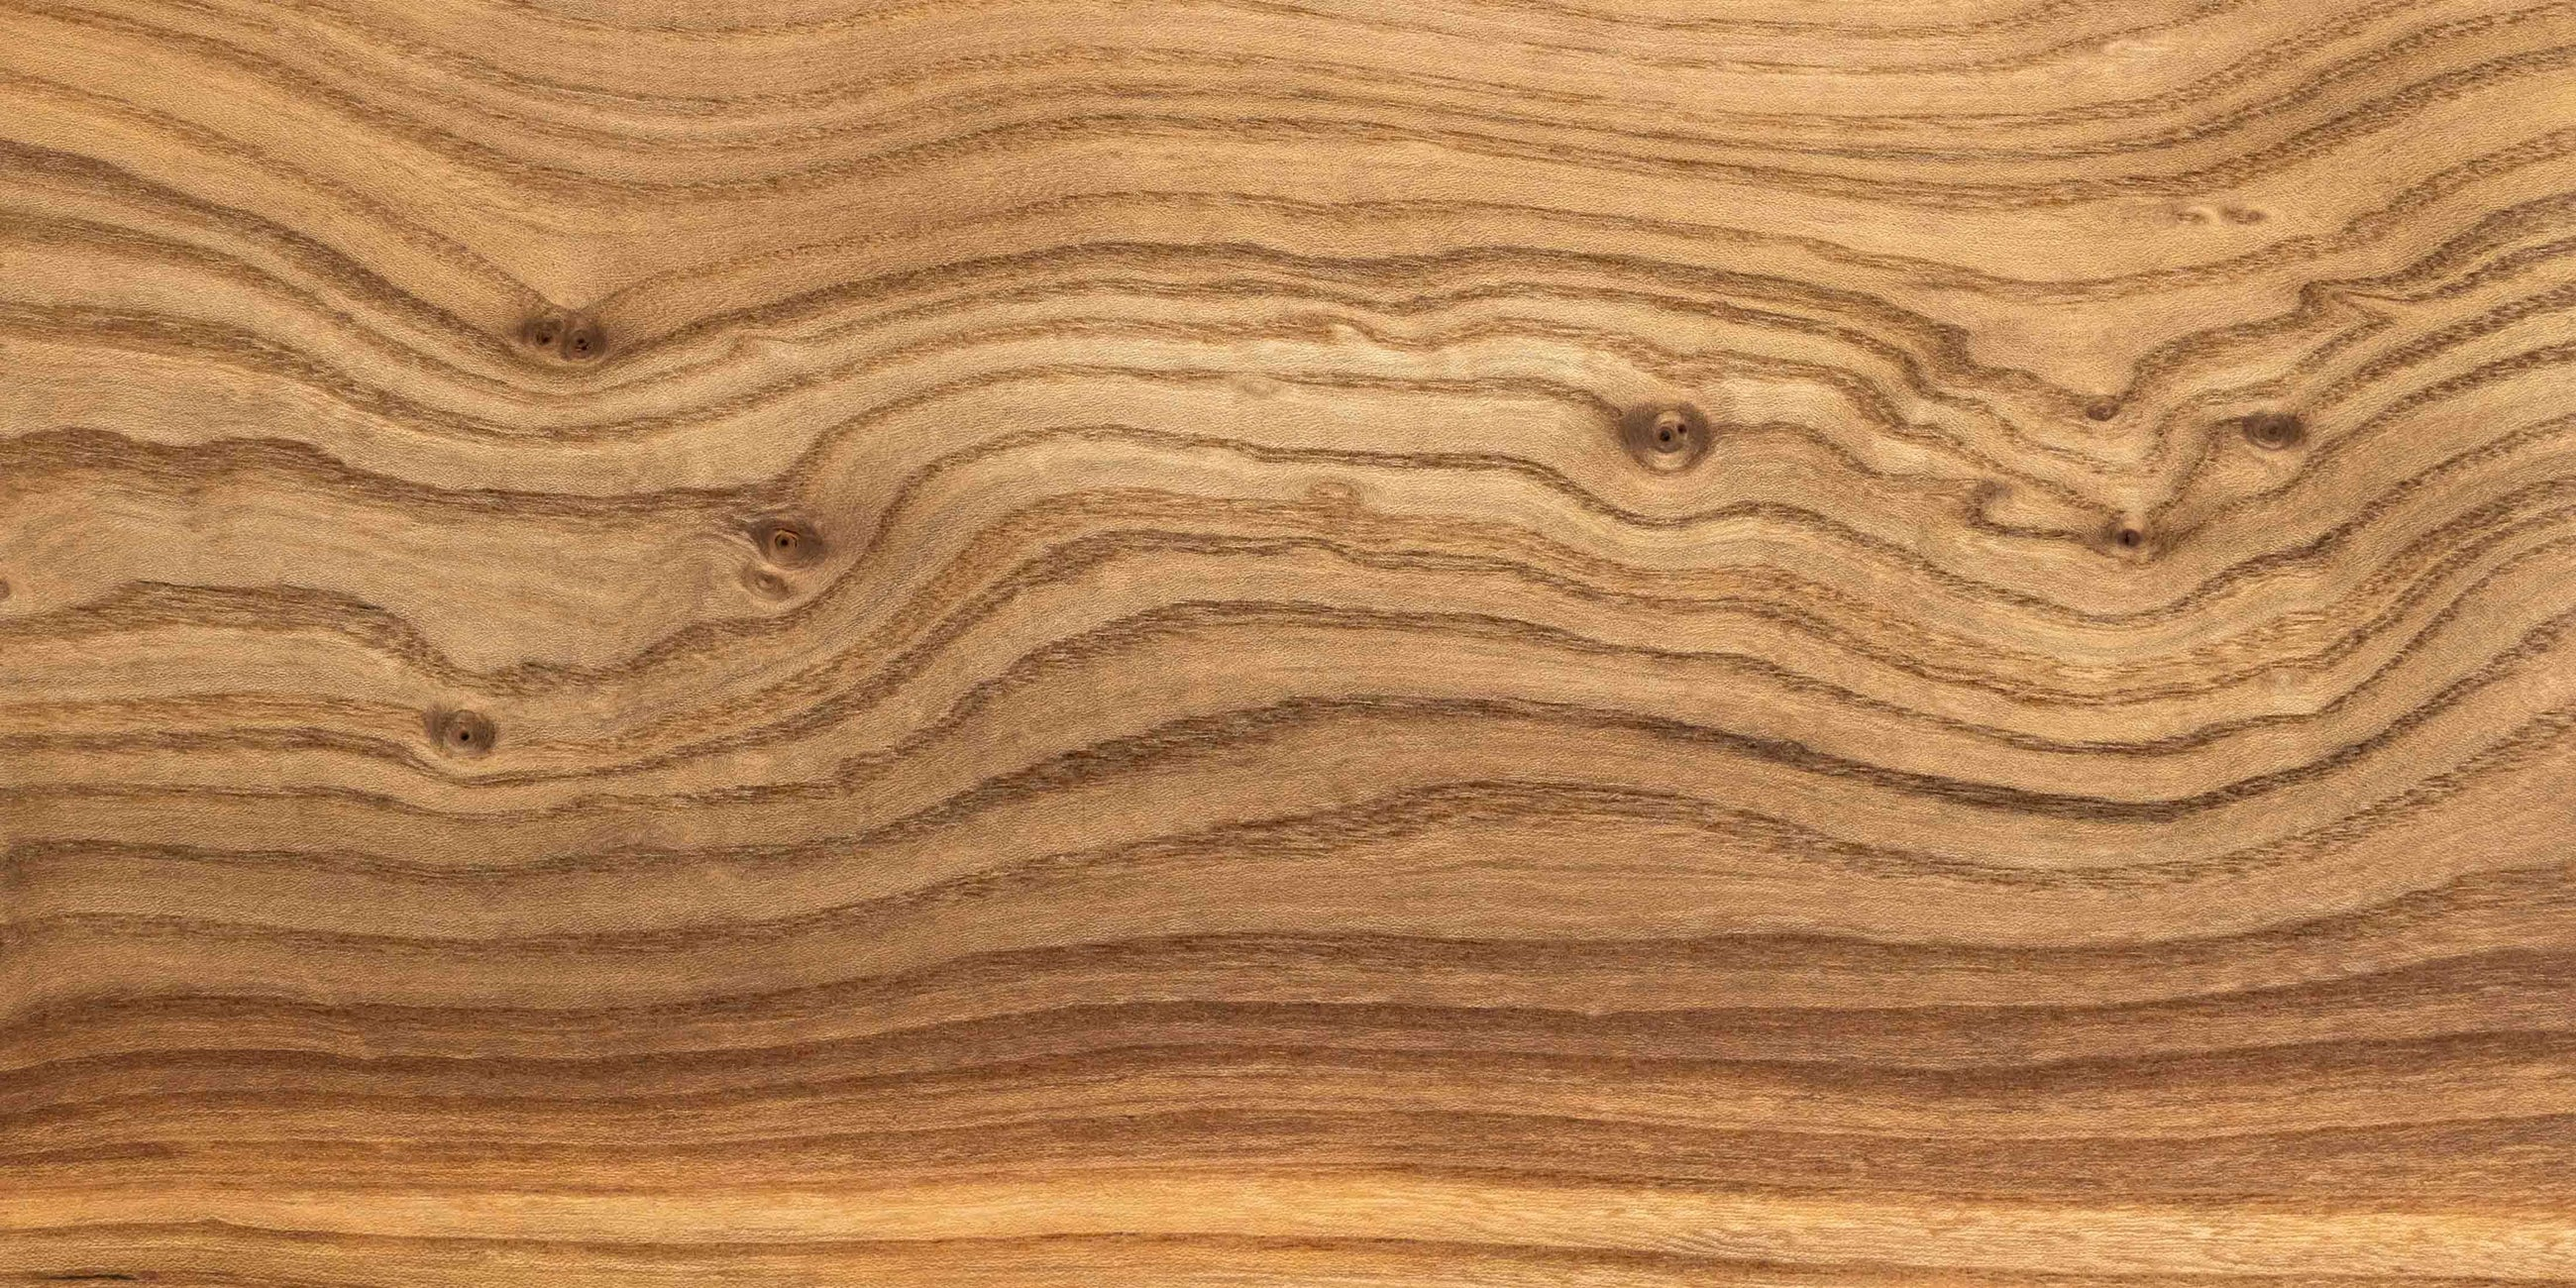
\includegraphics[width=0.8\linewidth]{images/wood.jpg}
          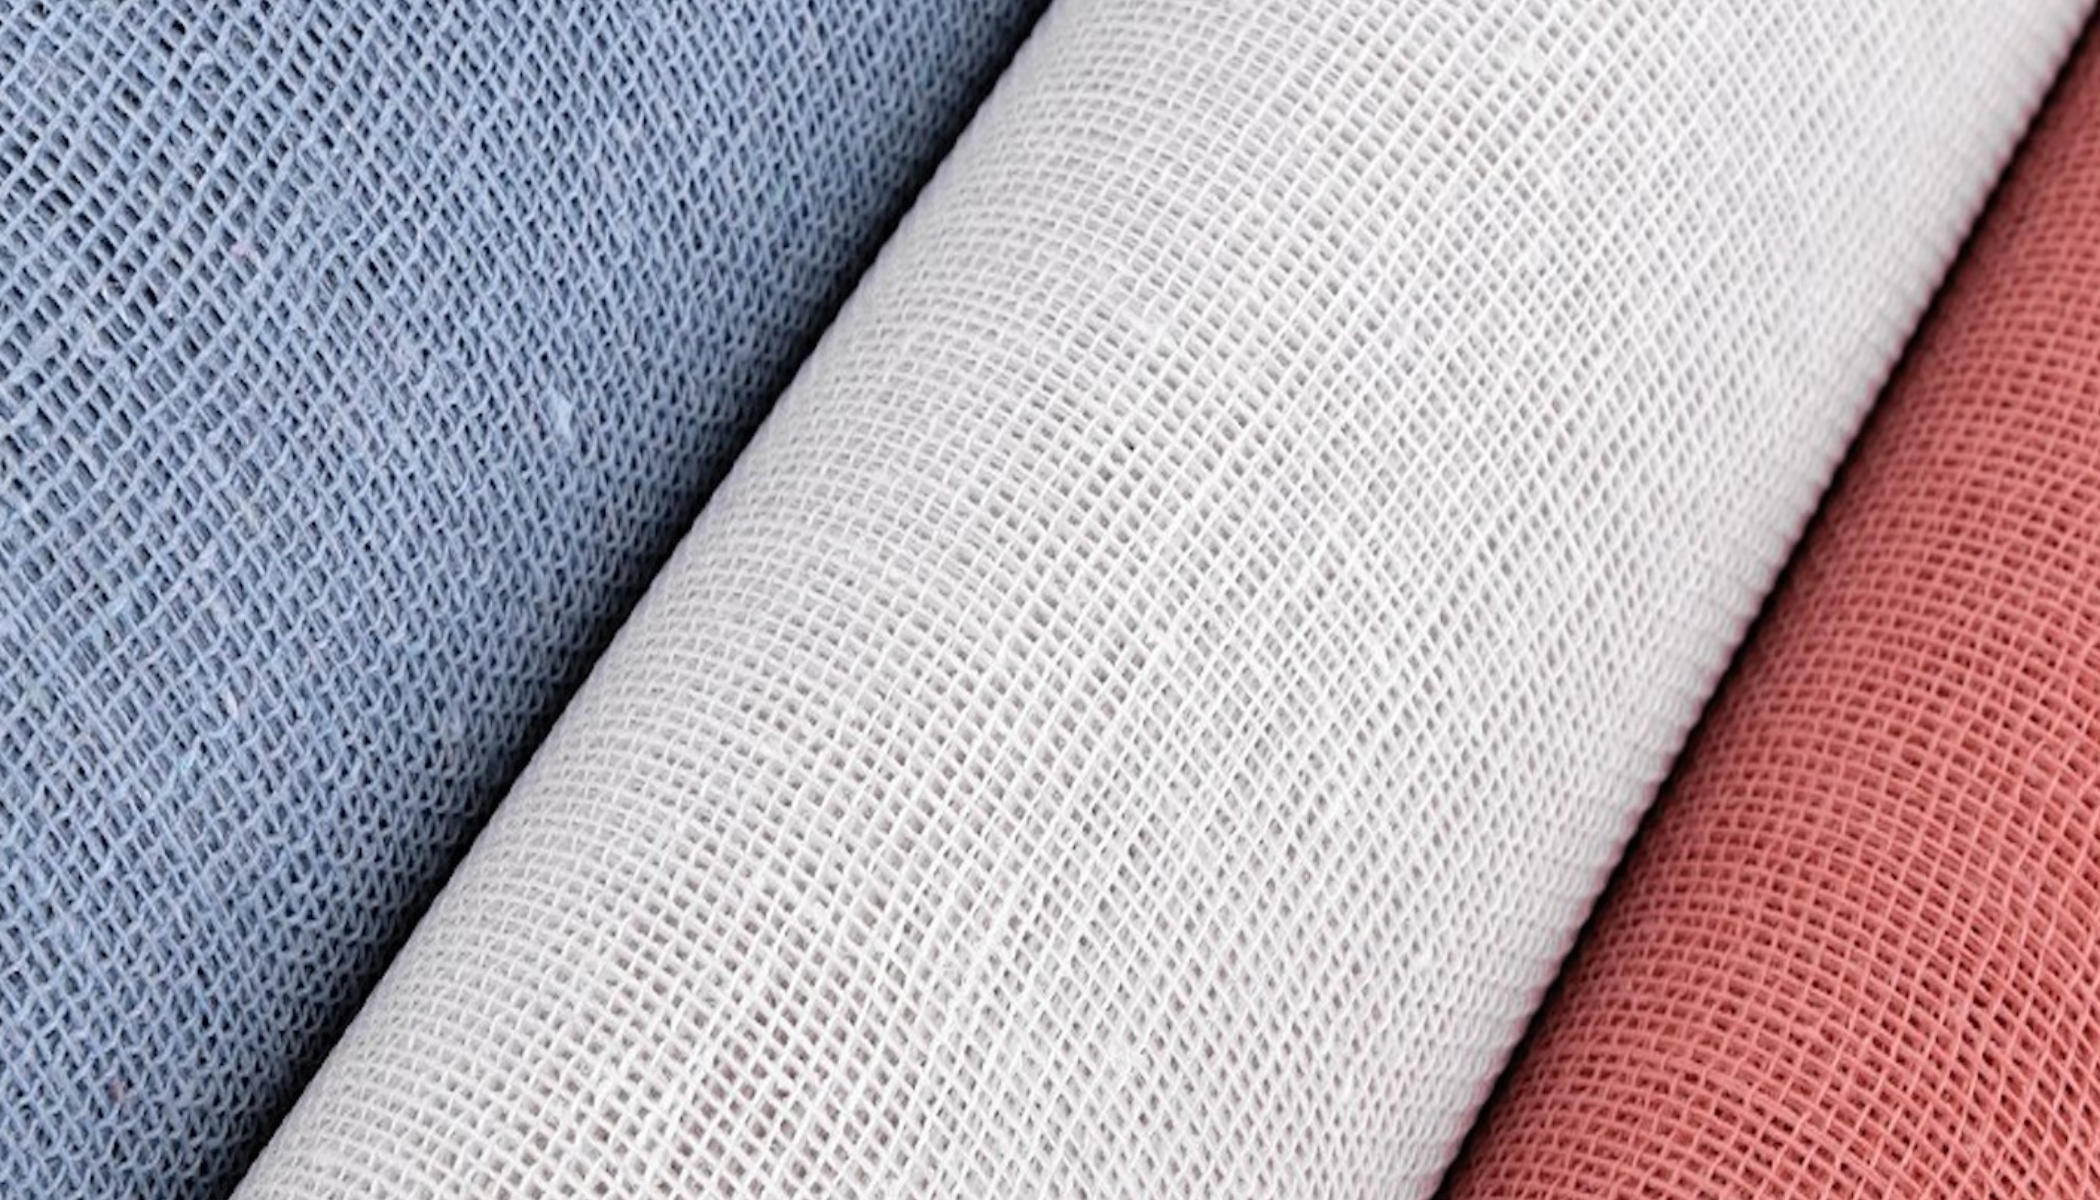
\includegraphics[width=0.8\linewidth]{images/fabric.png}
          \caption*{\scriptsize Examples of diffuse surfaces: wood and fabric}
        \end{figure}
      \end{center}
    \end{column}
  \end{columns}
\end{frame}

\begin{frame}{Lambert's Cosine Law - Intuition}
  \begin{columns}
    \begin{column}{0.5\textwidth}
      \begin{mathbox}{Why Cosine?}
        \footnotesize
        \textbf{Consider light hitting a surface:}

        \vspace{0.3cm}
        \pause
        \textbf{Energy per unit area depends on angle}

        When light hits at angle $\theta$:
        \begin{itemize}
          \item Same light beam covers larger area
          \item Energy density decreases
          \item Area increases by factor $1/\cos(\theta)$
          \item Energy density decreases by factor $\cos(\theta)$
        \end{itemize}

        \vspace{0.3cm}
        \pause
        \textbf{Mathematical relationship:}
        \begin{align*}
          \text{Effective intensity} \propto \cos(\theta) = \mathbf{N} \cdot \mathbf{L}
        \end{align*}
      \end{mathbox}
    \end{column}
    \begin{column}{0.4\textwidth}
      \centering
      \begin{tikzpicture}[scale=0.8]
        % Light beam hitting surface perpendicularly
        \draw[lightray, thick] (-0.5,2.5) -- (-0.5,1);
        \draw[lightray, thick] (0.5,2.5) -- (0.5,1);
        \draw[ObjectColor, very thick] (-1,1) -- (1,1);
        \node[below] at (0,0.7) {\footnotesize $\theta = 0^{\circ}$};
        \node[below] at (0,0.4) {\footnotesize Area = $A$};

        \draw[->, PrimaryColor] (0,1) -- (0,2);
        \begin{scope}[shift={(1,1.5)}]
          % Light beam hitting at angle
          \draw[lightray, thick] (-1,3.5) -- (0.5,2);
          \draw[lightray, thick] (0,3.5) -- (1.5,2);
          \draw[ObjectColor, very thick] (0,2) -- (2.5,2.5);

          % Angle indication
          \draw[dashed] (1.25,2.25) -- (1.25,3);
          \draw[dashed] (1.25,2.25) -- (0.5,3);
          \node[AccentColor] at (0.9,2.7) {\footnotesize $\theta$};

          \node[below] at (1.25,1.7) {\footnotesize Area = $A/\cos(\theta)$};
          \node[below] at (1.25,1.4) {\footnotesize Intensity $\times \cos(\theta)$};

          % Normal vectors
          \draw[->, PrimaryColor] (1.25,2.25) -- (0.75,3.25);
        \end{scope}
      \end{tikzpicture}
    \end{column}
  \end{columns}
\end{frame}

\begin{frame}{Diffuse Reflection - Mathematics}
  \begin{columns}
    \begin{column}{0.6\textwidth}
      \begin{mathbox}{Lambert's Law Implementation}
        \small
        \textbf{Diffuse component formula:}
        \begin{align*}
          I_{\text{diffuse}} = \mathbf{k}_d \odot \mathbf{I}_l (\mathbf{N} \cdot \mathbf{L})
        \end{align*}

        where:
        \begin{itemize}
          \item $\mathbf{k}_d$ = diffuse reflection coefficient (material color)
          \item $\mathbf{I}_l$ = intensity of the light source
          \item $\mathbf{N}$ = surface normal
          \item $\mathbf{L}$ = direction to light source
        \end{itemize}

        \pause
        \textbf{With Clamping:}
        \begin{align*}
          I_{\text{diffuse}} = \mathbf{k}_d \odot \mathbf{I}_l \max (0, \mathbf{N} \cdot \mathbf{L})
        \end{align*}
        To avoid negative lighting.
      \end{mathbox}
    \end{column}
    \begin{column}{0.4\textwidth}
      \only<3->{
        \begin{figure}
          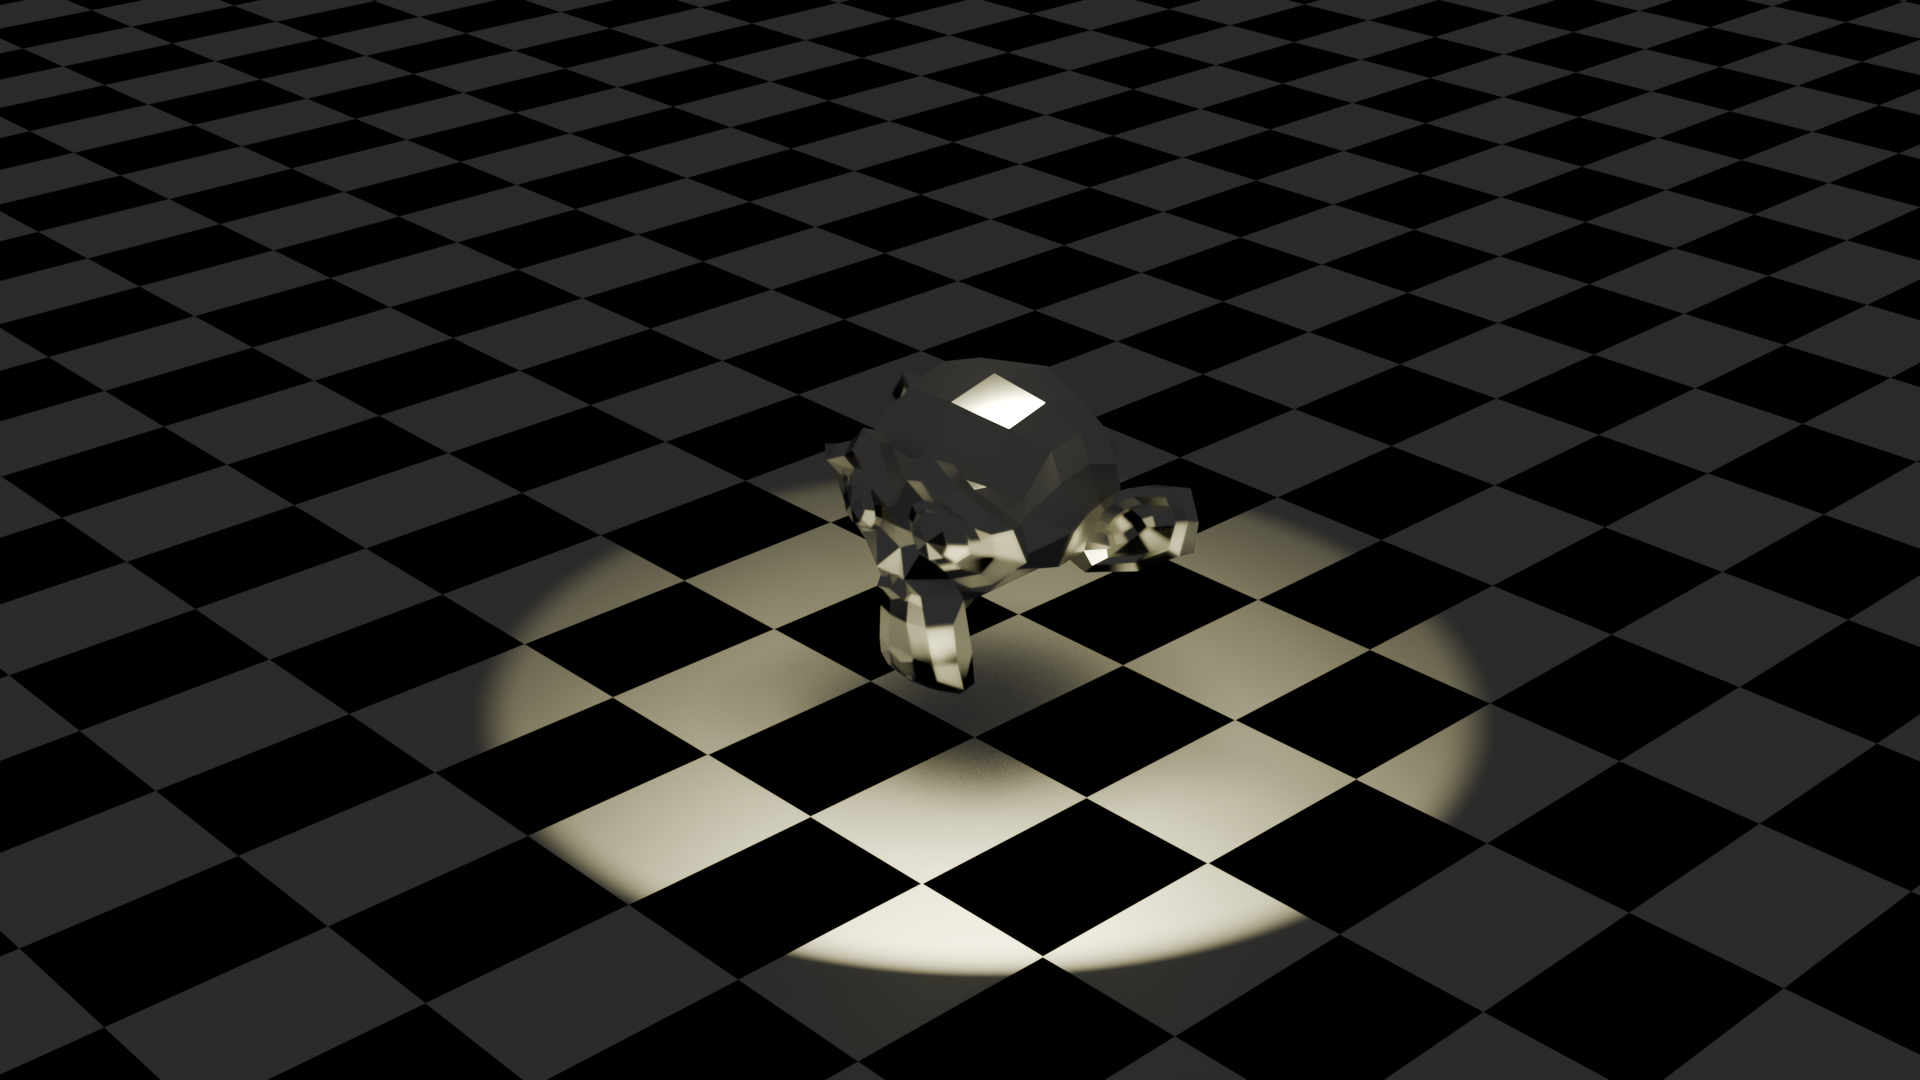
\includegraphics[width=\linewidth]{images/specular.png}
          \caption*{Low diffuse}
        \end{figure}
        \begin{figure}
          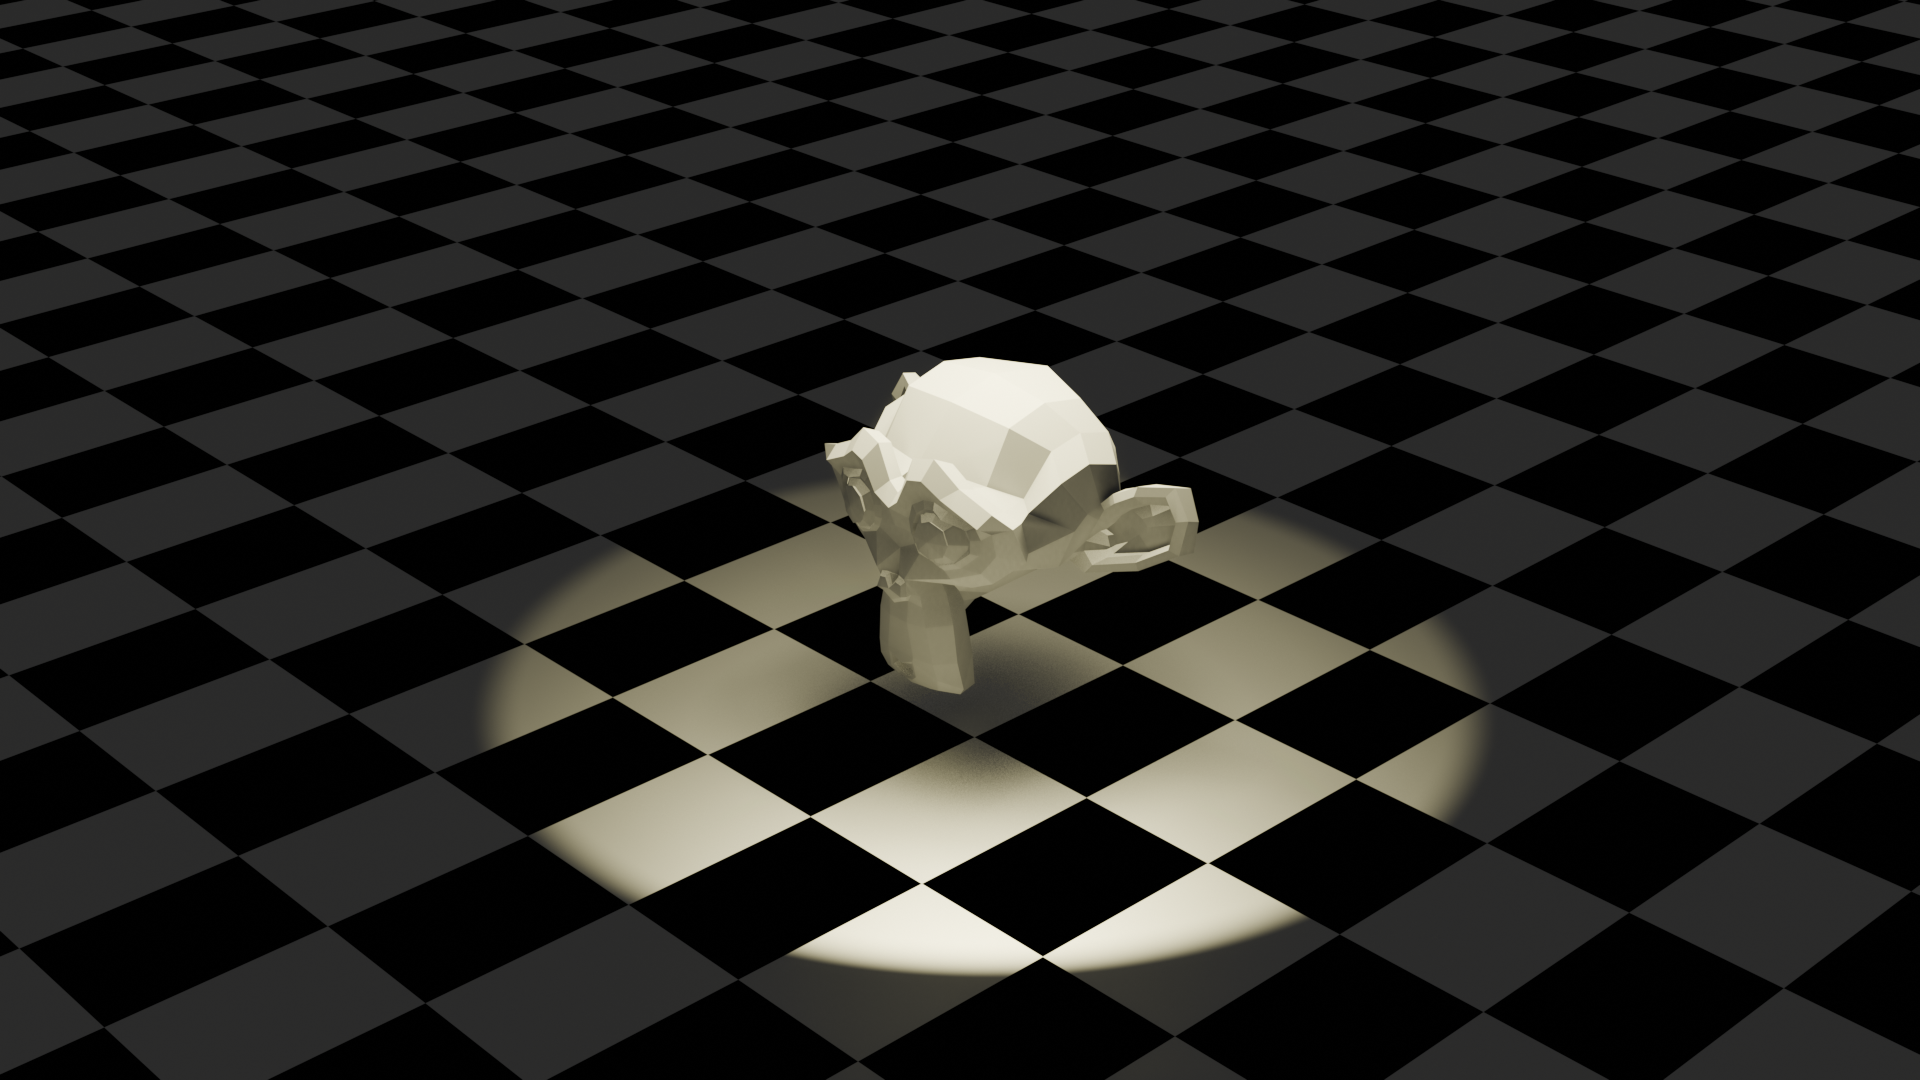
\includegraphics[width=\linewidth]{images/diffuse.png}
          \caption*{High diffuse}
        \end{figure}
      }
    \end{column}
  \end{columns}
\end{frame}
